\documentclass{article}
\usepackage[utf8]{inputenc}

\title{ASSIGNMENT-2}
\author{N.Soundarya}
\date{August 2022}
\usepackage{graphicx}
\begin{document}

\maketitle

\section{CIRCUIT}

For the logic circuit shown in Fig.P2.7, the simplified Boolean expression for the output is....\\
\begin{figure}
    \centering
    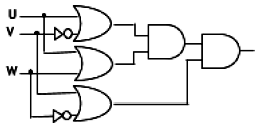
\includegraphics[width=4in]{1.PNG}
    \caption{F=U(V+!W)}
    \caption{circuit}
    \label{fig:circuit}
\end{figure}
\section{components}
\section{hardware}
\section{software}
ABSTARCT This manual shows how to use the 7447 BCD-
Seven Segment Display decoder to implement Boolean logic.



 \begin{table}[ht]
            \centering
            \begin{tabular}{|l|c|r|}
            \hline
        component & value & quantity\\
        \hline

Resistor & 220 & 1\\
\hline
Arduino & UNO & 1\\
\hline
Seven segment & - & 1\\
\hline
Decoder & 7447& 1\\
\hline
jumperwires & - & 1\\
\hline
breadboard & - & 1\\
\hline
\end{tabular}
\caption{First table}
\label{tab:first table}
\end{table}
\textbf{COMPONENTS}
...\\\
GIVEN CIRCUIT DIAGRAM \\
\textbf{Problem 2.1}. Make connections between the seven
segment display  and the 7447 IC using table 2\\
...\\
\textbf{HARDWARE}
 \begin{table}[ht]
            \centering
            \begin{tabular}{|l|c|c|c|c|c|c|r|}
            \hline
            7447 & !a & !b & !c & !d & !e & !f & !g
            \\hline
            display & a & b & c & d & e & f & g\\
            \hline
            \end{tabular}
\caption{second table}
\label{tab:second table}
\end{table}\\
\begin{figure}[ht]
\centering
\begin{minipage}[b]{.49\textwidth}
    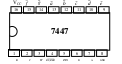
\includegraphics[width=2in]{7447ic.png}
    \caption{7447 pin diagram}
    \label{fig:7447 pin diagram}
     \end{minipage}
\begin{minipage}[b]{.49\textwidth}
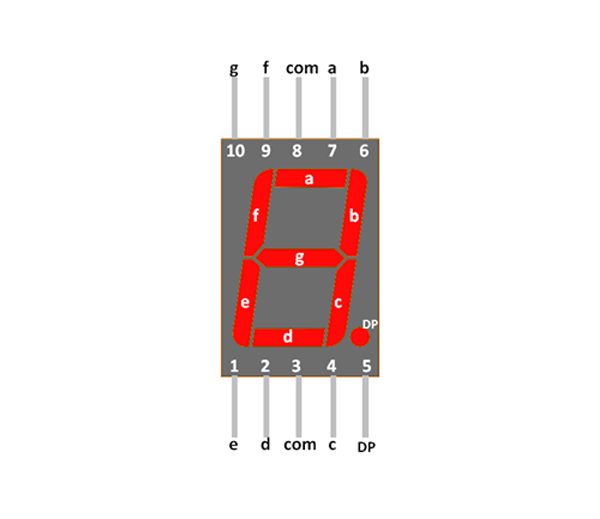
\includegraphics[width=2in]{seven segment.png}
    \caption{seven segment pin diagram}
    \label{fig:seven segment pin diagram}
     \end{minipage}
\end{figure}
...\\
X,Y,Z taken as inputs,connect arduino pin 2 to A in 7447,connect remaining B,C,D pins of 7447 to ground\\
Connect VCC (5 pin of arduino) and ground to the circuit
\\
\\
\\
\textbf{Execute the code provided in the below link}
\\
\\
https://github.com/soundaryanaru/FWC-assignments
\end{document}
